\documentclass[a4paper,12pt,twocolumn,landscape]{article}

\usepackage{superpack2015}

\usepackage[heightrounded]{geometry}	% heightrounded permet d'afficher les footers correctement
\geometry{hmargin=0.5cm,vmargin=1.5cm}

\setlength{\columnseprule}{0.5pt}		% Ligne séparatrice milieu document
\setlength{\columnsep}{50pt}			% Espace de chaque côté de la ligne
\setlength{\headsep}{15pt}
\addtolength{\textheight}{20pt}
%\setlength{\textwidth}{770pt}
%\setlength{\hoffset}{20pt}

\classichf
	% Nom du style
	{singlepage}
	% Hauteur sous header
	% 14.5pt si une ligne (1 \baselineskip)
	% 29.0pt si deux lignes (2 \baselineskip)
	{14.5pt}
	% Head
	{}
	{\textbf{Exercices : Repérage dans le plan}}
	{}
	% Foot
	{}
	{}
	{}

\classichf
	% Nom du style
	{doublepage}
	% Hauteur sous header
	% 14.5pt si une ligne (1 \baselineskip)
	% 29.0pt si deux lignes (2 \baselineskip)
	{14.5pt}
	% Head
	{\textbf{Exercices : Repérage dans le plan}}
	{}
	{\textbf{Exercices : Repérage dans le plan}}
	% Foot
	{}
	{}
	{}

%\usepackage{showframe}
%\usepackage{layout}

\begin{document}
%
% Exercices 1 et 2
%
\pagestyle{doublepage}	%\thispagestyle{premierepage} pour isoler des styles de pages
\exercice Lire les coordonnées des points suivants~: 
\begin{minipage}{0.35\textwidth}
\begin{center}
%\fbox{
\begin{tikzpicture}[scale=0.5,every node/.style={scale=0.5}]
	%Points
	\coordinate(A)at(3,1);
	\coordinate(B)at(5,5);
	\coordinate(C)at(4,3);
	\coordinate(D)at(4,-5);
	\coordinate(E)at(-7,4);
	\coordinate(F)at(-5,0);
	\coordinate(G)at(0,-3);
	\coordinate(H)at(0,7);
%
	\repereOIJ{-8}{8}{-8}{8};
%
	% Étiquettes
	\foreach \point in {A, ..., H}
		\draw(\point)node{$\times$};
	\foreach \point in {A, ..., H}
		\draw(\point)node[below right]{$\point$};	
	\foreach \r in {5}
    	\draw[thick, below right] (\r,0) node{\r};
	\foreach \r in {5}
    	\draw[thick, above left] (0,\r) node{\r};
\end{tikzpicture}
%}
\end{center}
\end{minipage}
\begin{minipage}{0.1\textwidth}
	\begin{enumerate}[]
		\item $A(~~~~~,~~~~~)$
		\item $B(~~~~~,~~~~~)$
		\item $C(~~~~~,~~~~~)$
		\item $D(~~~~~,~~~~~)$
		\item $E(~~~~~,~~~~~)$
		\item $F(~~~~~,~~~~~)$
		\item $G(~~~~~,~~~~~)$
		\item $H(~~~~~,~~~~~)$
	\end{enumerate}
\end{minipage}
\exercice Placer un point connaissant ses coordonnées~:
\begin{minipage}{0.35\textwidth}
\begin{center}
%\fbox{
\begin{tikzpicture}[scale=0.5,every node/.style={scale=0.5}]
	%Points
	\coordinate(A)at(5,3);
	\coordinate(B)at(-2,3);
	\coordinate(C)at(-2,-4);
	\coordinate(D)at(6,2);
	\coordinate(E)at(7,-4);
	\coordinate(F)at(6,0);
	\coordinate(G)at(0,3);
	\coordinate(H)at(0,-7);
%
	\repereOIJ{-8}{8}{-8}{8};
%
	% Étiquettes
%
%	Réponses
%	\foreach \point in {A, ..., H}
%		\draw(\point)node{$\times$};
%	\foreach \point in {A, ..., H}
%		\draw(\point)node[below right]{$\point$};	
	\foreach \r in {5}
    	\draw[thick, below right] (\r,0) node{\r};
	\foreach \r in {5}
    	\draw[thick, above left] (0,\r) node{\r};
\end{tikzpicture}
%}
\end{center}
\end{minipage}
\begin{minipage}{0.1\textwidth}
	\begin{enumerate}[]
		\item $A(~~5~,~3~)$
		\item $B(~-2~,~3~)$
		\item $C(-2,-4)$
		\item $D(~~6~,~~2~)$
		\item $E(~~7~,~-4)$
		\item $F(~~6~,~~0~)$
		\item $G(~~0~,~~3~)$
		\item $H(~~0~,-7)$
	\end{enumerate}
\end{minipage}

\newpage
\addtocounter{exercice}{-2}
\exercice Lire les coordonnées des points suivants~: 
\begin{minipage}{0.35\textwidth}
\begin{center}
%\fbox{
\begin{tikzpicture}[scale=0.5,every node/.style={scale=0.5}]
	%Points
	\coordinate(A)at(3,1);
	\coordinate(B)at(5,5);
	\coordinate(C)at(4,3);
	\coordinate(D)at(4,-5);
	\coordinate(E)at(-7,4);
	\coordinate(F)at(-5,0);
	\coordinate(G)at(0,-3);
	\coordinate(H)at(0,7);
%
	\repereOIJ{-8}{8}{-8}{8};
%
	% Étiquettes
	\foreach \point in {A, ..., H}
		\draw(\point)node{$\times$};
	\foreach \point in {A, ..., H}
		\draw(\point)node[below right]{$\point$};	
	\foreach \r in {5}
    	\draw[thick, below right] (\r,0) node{\r};
	\foreach \r in {5}
    	\draw[thick, above left] (0,\r) node{\r};
\end{tikzpicture}
%}
\end{center}
\end{minipage}
\begin{minipage}{0.1\textwidth}
	\begin{enumerate}[]
		\item $A(~~~~~,~~~~~)$
		\item $B(~~~~~,~~~~~)$
		\item $C(~~~~~,~~~~~)$
		\item $D(~~~~~,~~~~~)$
		\item $E(~~~~~,~~~~~)$
		\item $F(~~~~~,~~~~~)$
		\item $G(~~~~~,~~~~~)$
		\item $H(~~~~~,~~~~~)$
	\end{enumerate}
\end{minipage}
\exercice Placer un point connaissant ses coordonnées~:
\begin{minipage}{0.35\textwidth}
\begin{center}
%\fbox{
\begin{tikzpicture}[scale=0.5,every node/.style={scale=0.5}]
	%Points
	\coordinate(A)at(5,3);
	\coordinate(B)at(-2,3);
	\coordinate(C)at(-2,-4);
	\coordinate(D)at(6,2);
	\coordinate(E)at(7,-4);
	\coordinate(F)at(6,0);
	\coordinate(G)at(0,3);
	\coordinate(H)at(0,-7);
%
	\repereOIJ{-8}{8}{-8}{8};
%
	% Étiquettes
%
%	Réponses
%	\foreach \point in {A, ..., H}
%		\draw(\point)node{$\times$};
%	\foreach \point in {A, ..., H}
%		\draw(\point)node[below right]{$\point$};	
	\foreach \r in {5}
    	\draw[thick, below right] (\r,0) node{\r};
	\foreach \r in {5}
    	\draw[thick, above left] (0,\r) node{\r};
\end{tikzpicture}
%}
\end{center}
\end{minipage}
\begin{minipage}{0.1\textwidth}
	\begin{enumerate}[]
		\item $A(~~5~,~3~)$
		\item $B(~-2~,~3~)$
		\item $C(-2,-4)$
		\item $D(~~6~,~~2~)$
		\item $E(~~7~,~-4)$
		\item $F(~~6~,~~0~)$
		\item $G(~~0~,~~3~)$
		\item $H(~~0~,-7)$
	\end{enumerate}
\end{minipage}

\newpage
%
% Exercice 3
%
\pagestyle{doublepage}	%\thispagestyle{premierepage} pour isoler des styles de pages
\input{geometrie1-td-exercice2}
\newpage
\addtocounter{exercice}{-1}
\input{geometrie1-td-exercice2}
%
% Exercice 4
%
\newpage
\exercice Donner les coordonnées des points dans les repères ci-dessous~:

\begin{minipage}{0.35\textwidth}
		\begin{tikzpicture}[scale=0.5,every node/.style={scale=0.5}]
		%Points
		\coordinate(O)at(0,0);
		\coordinate(I)at(1,0);
		\coordinate(J)at(0,1);
		\coordinate(xstart)at(-8,0);
		\coordinate(xend)at(8,0);
		\coordinate(ystart)at(0,-8);
		\coordinate(yend)at(0,8);
		\coordinate(A)at(-2,-1);
		\coordinate(B)at(-7,4);
		\coordinate(C)at(4,-5);
		\coordinate(D)at(-3,-4);
		\coordinate(E)at(3,4);
		\coordinate(F)at(-5,1);
		\coordinate(G)at(1,-3);
		\coordinate(H)at(-2,7);
		%Étiquettes
	%	\draw (I) node[below right] {$1$};
	%	\draw (J) node[above left] {$1$};
		\draw (xend) node[below right] {$x$};
		\draw (yend) node[above left] {$y$};	
		%%%%%%%%%%%%%%%%%%%%%%%%%%%%%%%%%%%%
		%Axes
		\draw [thick] (xstart) -- (xend);
		\draw [thick] (ystart) -- (yend);
		%Flèches
	%	\draw [>=stealth,->] (O) -- (I);
	%	\draw [>=stealth,->] (O) -- (J);
		\draw [>=stealth,->] (O) -- (xend);
		\draw [>=stealth,->] (O) -- (yend);
	%	%Grille
	%	\draw [thin] (-8,-8)grid(8,8);
		%%%%%%%%%%%%%%%%%%%%%%%%%%%%%%%%%%%%
		%étiquettes
		\foreach \point in {A, ..., H}
			\draw(\point)node{$\times$};
		\foreach \point in {A, ..., H}
			\draw(\point)node[below right]{$\point$};		
		\foreach \r in {-7, -6, ..., 7}
	    	\draw[thick, below right] (\r,0) node{\r};
		\foreach \r in {-7, -6, ..., 7}
	    	\draw[thick, above left] (0,\r) node{\r};  
		\foreach \r in {-7, -6, ..., 7}
	    	\draw[thick] (\r,0) node{$|$};
		\foreach \r in {-7, -6, ..., 7}
	    	\draw[thick] (0,\r) node{$--$};
	   	\foreach \r in {-6, -4, ..., 6}
	    	\draw[dashed] (-8,\r)--(8,\r);
	   	\foreach \r in {-6, -4, ..., 6}
	    	\draw[dashed] (\r,-8)--(\r,8);
	%	\foreach \r in {0, 1,...,7}
	%    	\draw[thick, below right] (\r,0) node{\r};
	\end{tikzpicture}

\end{minipage}
\begin{minipage}{0.1\textwidth}
	\begin{enumerate}[]
		\item $\pointcoord{A}{~~~~}{~~~~}$
		\item $\pointcoord{B}{~~~~}{~~~~}$
		\item $\pointcoord{C}{~~~~}{~~~~}$
		\item $\pointcoord{D}{~~~~}{~~~~}$
		\item $\pointcoord{E}{~~~~}{~~~~}$
		\item $\pointcoord{F}{~~~~}{~~~~}$
		\item $\pointcoord{G}{~~~~}{~~~~}$
		\item $\pointcoord{H}{~~~~}{~~~~}$
	\end{enumerate}
\end{minipage}

\vspace{2em}

\begin{minipage}{0.35\textwidth}
				\begin{tikzpicture}[line cap=round,line join=round,>=triangle 45,x=1.0cm,y=1.0cm,scale=1,every node/.style={scale=1}]
			
			\tikzstyle{tiret}=[dash pattern=on 3pt off 3pt];
			\tikzstyle{domaine}=[domain=-5:8];
			\clip(-3.5,-2.5) rectangle (5.5,2.5);
			\draw [domaine] plot(\x,{(-0-0*\x)/1});
			\draw [domaine] plot(\x,{(-0--1*\x)/1});
			\draw [tiret,domaine] plot(\x,{(-1--1*\x)/1});
			\draw [tiret,domaine] plot(\x,{(-2--1*\x)/1});
			\draw [tiret,domaine] plot(\x,{(-3--1*\x)/1});
			\draw [tiret,domaine] plot(\x,{(-4--1*\x)/1});
			\draw [tiret,domaine] plot(\x,{(-5--1*\x)/1});
			\draw [tiret,domaine] plot(\x,{(--1--1*\x)/1});
			\draw [tiret,domaine] plot(\x,{(--2--1*\x)/1});
			\draw [tiret,domaine] plot(\x,{(--3--1*\x)/1});
			\draw [tiret,domaine] plot(\x,{(--1-0*\x)/1});
			\draw [tiret,domaine] plot(\x,{(--2-0*\x)/1});
			\draw [tiret,domaine] plot(\x,{(-1-0*\x)/1});
			\draw [tiret,domaine] plot(\x,{(-2-0*\x)/1});
			\draw [tiret,domaine] plot(\x,{(--4--1*\x)/1});
			\draw [tiret,domaine] plot(\x,{(-6--1*\x)/1});
			\draw [domaine] plot(\x,{(-0-0*\x)/-1});
			\draw [domaine] plot(\x,{(-0-0*\x)/-1});
			\draw [domaine] plot(\x,{(-0-0*\x)/-1});
			\begin{scriptsize}
			\draw (0,0) node {$\times$} node[above left] {$A$};
			\draw (1,0) node {$\times$} node[above left] {$I$};
			\draw (1,1) node {$\times$} node[above left] {$J$};
			\draw (3,0) node {$\times$} node[above left] {$E$};
			\draw (5,2) node {$\times$} node[above left] {$F$};
			\draw (1,-1) node {$\times$} node[above left] {$D$};
			\draw (-2,-2) node {$\times$} node[above left] {$C$};
			\draw (-2,2) node {$\times$} node[above left] {$B$};
			\draw (-3,0) node {$\times$} node[above left] {$G$};
			\draw (-3,-1) node {$\times$} node[above left] {$H$};
			\end{scriptsize}
			\end{tikzpicture}

\end{minipage}
\begin{minipage}{0.1\textwidth}
	\begin{enumerate}[]
		\item $\pointcoord{A}{~~~~}{~~~~}$
		\item $\pointcoord{B}{~~~~}{~~~~}$
		\item $\pointcoord{C}{~~~~}{~~~~}$
		\item $\pointcoord{D}{~~~~}{~~~~}$
		\item $\pointcoord{E}{~~~~}{~~~~}$
		\item $\pointcoord{F}{~~~~}{~~~~}$
		\item $\pointcoord{G}{~~~~}{~~~~}$
		\item $\pointcoord{H}{~~~~}{~~~~}$
	\end{enumerate}
\end{minipage}


\newpage
\addtocounter{exercice}{-1}
\exercice Donner les coordonnées des points dans les repères ci-dessous~:

\begin{minipage}{0.35\textwidth}
		\begin{tikzpicture}[scale=0.5,every node/.style={scale=0.5}]
		%Points
		\coordinate(O)at(0,0);
		\coordinate(I)at(1,0);
		\coordinate(J)at(0,1);
		\coordinate(xstart)at(-8,0);
		\coordinate(xend)at(8,0);
		\coordinate(ystart)at(0,-8);
		\coordinate(yend)at(0,8);
		\coordinate(A)at(-2,-1);
		\coordinate(B)at(-7,4);
		\coordinate(C)at(4,-5);
		\coordinate(D)at(-3,-4);
		\coordinate(E)at(3,4);
		\coordinate(F)at(-5,1);
		\coordinate(G)at(1,-3);
		\coordinate(H)at(-2,7);
		%Étiquettes
	%	\draw (I) node[below right] {$1$};
	%	\draw (J) node[above left] {$1$};
		\draw (xend) node[below right] {$x$};
		\draw (yend) node[above left] {$y$};	
		%%%%%%%%%%%%%%%%%%%%%%%%%%%%%%%%%%%%
		%Axes
		\draw [thick] (xstart) -- (xend);
		\draw [thick] (ystart) -- (yend);
		%Flèches
	%	\draw [>=stealth,->] (O) -- (I);
	%	\draw [>=stealth,->] (O) -- (J);
		\draw [>=stealth,->] (O) -- (xend);
		\draw [>=stealth,->] (O) -- (yend);
	%	%Grille
	%	\draw [thin] (-8,-8)grid(8,8);
		%%%%%%%%%%%%%%%%%%%%%%%%%%%%%%%%%%%%
		%étiquettes
		\foreach \point in {A, ..., H}
			\draw(\point)node{$\times$};
		\foreach \point in {A, ..., H}
			\draw(\point)node[below right]{$\point$};		
		\foreach \r in {-7, -6, ..., 7}
	    	\draw[thick, below right] (\r,0) node{\r};
		\foreach \r in {-7, -6, ..., 7}
	    	\draw[thick, above left] (0,\r) node{\r};  
		\foreach \r in {-7, -6, ..., 7}
	    	\draw[thick] (\r,0) node{$|$};
		\foreach \r in {-7, -6, ..., 7}
	    	\draw[thick] (0,\r) node{$--$};
	   	\foreach \r in {-6, -4, ..., 6}
	    	\draw[dashed] (-8,\r)--(8,\r);
	   	\foreach \r in {-6, -4, ..., 6}
	    	\draw[dashed] (\r,-8)--(\r,8);
	%	\foreach \r in {0, 1,...,7}
	%    	\draw[thick, below right] (\r,0) node{\r};
	\end{tikzpicture}

\end{minipage}
\begin{minipage}{0.1\textwidth}
	\begin{enumerate}[]
		\item $\pointcoord{A}{~~~~}{~~~~}$
		\item $\pointcoord{B}{~~~~}{~~~~}$
		\item $\pointcoord{C}{~~~~}{~~~~}$
		\item $\pointcoord{D}{~~~~}{~~~~}$
		\item $\pointcoord{E}{~~~~}{~~~~}$
		\item $\pointcoord{F}{~~~~}{~~~~}$
		\item $\pointcoord{G}{~~~~}{~~~~}$
		\item $\pointcoord{H}{~~~~}{~~~~}$
	\end{enumerate}
\end{minipage}

\vspace{2em}

\begin{minipage}{0.35\textwidth}
				\begin{tikzpicture}[line cap=round,line join=round,>=triangle 45,x=1.0cm,y=1.0cm,scale=1,every node/.style={scale=1}]
			
			\tikzstyle{tiret}=[dash pattern=on 3pt off 3pt];
			\tikzstyle{domaine}=[domain=-5:8];
			\clip(-3.5,-2.5) rectangle (5.5,2.5);
			\draw [domaine] plot(\x,{(-0-0*\x)/1});
			\draw [domaine] plot(\x,{(-0--1*\x)/1});
			\draw [tiret,domaine] plot(\x,{(-1--1*\x)/1});
			\draw [tiret,domaine] plot(\x,{(-2--1*\x)/1});
			\draw [tiret,domaine] plot(\x,{(-3--1*\x)/1});
			\draw [tiret,domaine] plot(\x,{(-4--1*\x)/1});
			\draw [tiret,domaine] plot(\x,{(-5--1*\x)/1});
			\draw [tiret,domaine] plot(\x,{(--1--1*\x)/1});
			\draw [tiret,domaine] plot(\x,{(--2--1*\x)/1});
			\draw [tiret,domaine] plot(\x,{(--3--1*\x)/1});
			\draw [tiret,domaine] plot(\x,{(--1-0*\x)/1});
			\draw [tiret,domaine] plot(\x,{(--2-0*\x)/1});
			\draw [tiret,domaine] plot(\x,{(-1-0*\x)/1});
			\draw [tiret,domaine] plot(\x,{(-2-0*\x)/1});
			\draw [tiret,domaine] plot(\x,{(--4--1*\x)/1});
			\draw [tiret,domaine] plot(\x,{(-6--1*\x)/1});
			\draw [domaine] plot(\x,{(-0-0*\x)/-1});
			\draw [domaine] plot(\x,{(-0-0*\x)/-1});
			\draw [domaine] plot(\x,{(-0-0*\x)/-1});
			\begin{scriptsize}
			\draw (0,0) node {$\times$} node[above left] {$A$};
			\draw (1,0) node {$\times$} node[above left] {$I$};
			\draw (1,1) node {$\times$} node[above left] {$J$};
			\draw (3,0) node {$\times$} node[above left] {$E$};
			\draw (5,2) node {$\times$} node[above left] {$F$};
			\draw (1,-1) node {$\times$} node[above left] {$D$};
			\draw (-2,-2) node {$\times$} node[above left] {$C$};
			\draw (-2,2) node {$\times$} node[above left] {$B$};
			\draw (-3,0) node {$\times$} node[above left] {$G$};
			\draw (-3,-1) node {$\times$} node[above left] {$H$};
			\end{scriptsize}
			\end{tikzpicture}

\end{minipage}
\begin{minipage}{0.1\textwidth}
	\begin{enumerate}[]
		\item $\pointcoord{A}{~~~~}{~~~~}$
		\item $\pointcoord{B}{~~~~}{~~~~}$
		\item $\pointcoord{C}{~~~~}{~~~~}$
		\item $\pointcoord{D}{~~~~}{~~~~}$
		\item $\pointcoord{E}{~~~~}{~~~~}$
		\item $\pointcoord{F}{~~~~}{~~~~}$
		\item $\pointcoord{G}{~~~~}{~~~~}$
		\item $\pointcoord{H}{~~~~}{~~~~}$
	\end{enumerate}
\end{minipage}


%
% Exercice 5, 6, 7 et 8
%
\newpage
\pagestyle{singlepage}
\exercice \\

\begin{minipage}{0.25\textwidth}
\begin{center}
%\fbox{
\begin{tikzpicture}[scale=1.8,every node/.style={scale=0.7}]
	%Points
	\coordinate(A)at(-1,0);
	\coordinate(B)at(-1,-1);
	\coordinate(C)at(0,-1);
	\coordinate(D)at(0,0);
	\coordinate(E)at(0,1);
	\coordinate(F)at(-1,1);
	\coordinate(G)at(1,0);
	\coordinate(H)at(1,1);
	\coordinate(I)at(2,0);
	\coordinate(J)at(-1,2);
	\draw (A)--(B)--(C)--(D)--cycle;
	\draw (A)--(D)--(E)--(F)--cycle;
	\draw (D)--(G)--(H)--(E)--cycle;
	\draw (F)--(J);
	\draw (C)--(G);
	\draw (G)--(I);
	\draw (H)--(I);
	%Étiquettes
	\foreach \point in {A, ..., G, I, J}
		\draw(\point)node{$\times$};
	\foreach \point in {A, ..., G, I, J}
		\draw(\point)node[below right]{$\point$};
	\foreach \point in {H}
		\draw(\point)node{$\times$};
	\foreach \point in {H}
		\draw(\point)node[above right]{$\point$};
\end{tikzpicture}
%}
\end{center}
\end{minipage}
\begin{minipage}{0.2\textwidth}
$BCDA$, $ADEF$ et $DGHE$ sont des carrés de côté $1$.
~\\~\\
De plus le point $I$ est sur la droite $(AG)$ avec $GI = 1$ et le point $J$ sur la droite $(BF)$ avec $FJ = 1$.

\end{minipage}


\begin{enumerate}
	\item Déterminer les coordonnées de tous les points de la figure
	\begin{enumerate}
		\item dans le repère $(D, G, E)$ qui est orthonormé.
		\item dans le repère $(A, G, J)$ qui est aussi orthonormé.
	\end{enumerate}
~\\
\textbf{A partir de maintenant on n’utilisera que le repère $\mathbf{\left(D, G, E\right)}$.}

	\item Déterminer dans ce repère les coordonnées des points
	\begin{enumerate}
		\item $K$ milieu de $\left[CI\right]$
		\item $L$ milieu de $\left[HJ\right]$.
	\end{enumerate}

	\item Le quadrilatère $FLIK$ est-il un parallélogramme ? Justifier.

	\item Déterminer les coordonnées des points
	\begin{enumerate}
		\item $M$ milieu de $\left[AL\right]$
		\item $N$ milieu de $\left[GI\right]$.
	\end{enumerate}
	Le quadrilatère MLNK est-il un parallélogramme ? Justifier.
	\item Déterminer les coordonnées du point $P$ milieu de $\left[FN\right]$ puis du point $O$ tel que $FLNO$ soit un parallélogramme.
	\item Calculer les longueurs des diagonales $FN$ et $LO$ de ce parallélogramme.
	\item Le triangle $FLK$ est-il rectangle ?
	\item Les points $A$, $O$, $G$ et $H$ sont-ils situés sur un même cercle ?
\end{enumerate}


\exercice

\begin{minipage}{0.25\textwidth}
\begin{center}
%\fbox{
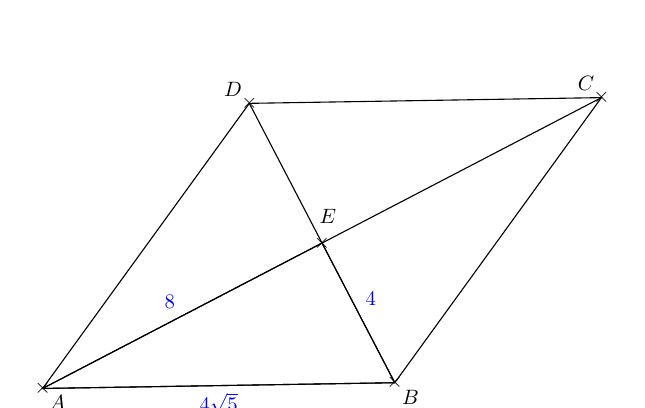
\begin{tikzpicture}[scale=0.5,every node/.style={scale=0.75}]
	%Points
	\begin{scope}[rotate=-62.5]
	\coordinate(A)at(0,0);
	\coordinate(B)at(4,8);
	\coordinate(C)at(0,16);
	\coordinate(D)at(-4,8);
	\coordinate(E)at(0,8);
%	\coordinate(F)at(-1,1);
%	\coordinate(G)at(1,0);
%	\coordinate(H)at(1,1);
%	\coordinate(I)at(2,0);
%	\coordinate(J)at(-1,2);
	\draw (A)--(B)--(C)--(D)--cycle;
	\draw (A)--(C);
	\draw (B)--(D);
	\draw (A)--(E) node[midway, above left, blue]{$8$};
	\draw (B)--(E) node[midway, above right, blue]{$4$};
	\draw (A)--(B) node[midway, below, blue]{$4\sqrt{5}$};
	%Étiquettes
	\foreach \point in {A, B}
		\draw(\point)node{$\times$};
	\foreach \point in {A, B}
		\draw(\point)node[below right]{$\point$};
	\foreach \point in {E}
		\draw(\point)node{$\times$};
	\foreach \point in {E}
		\draw(\point)node[above,shift={(0.1,0.2)}]{$\point$};
	\foreach \point in {C, D}
		\draw(\point)node{$\times$};
	\foreach \point in {C, D}
		\draw(\point)node[above left]{$\point$};
%	\foreach \point in {H}
%		\draw(\point)node{$\times$};
%	\foreach \point in {H}
%		\draw(\point)node[above right]{$\point$};
	\end{scope}
\end{tikzpicture}
%}
\end{center}
\end{minipage}
\begin{minipage}{0.2\textwidth}
Le parallélogramme ci-contre est-il un losange~?
\end{minipage}


\exercice\\

$ABC$ est un triangle isocèle en $A$.\\
Le cercle $\mathscr{C}$ , de diamètre $[AB]$, coupe $[BC]$ en $D$ et $[AC]$ en $E$.\\
La perpendiculaire à $(AB)$ passant par $C$ coupe la droite $(BE)$ en $F$.\\

\textbf{Objectif :} Démontrer que $A$, $D$ et $F$ sont alignés, et que $(AF)$ est la médiatrice de $[BC]$.\\

\begin{enumerate}
	\item Faire une figure.
	\item	\begin{enumerate} 
				\item Quelle est la nature des triangles $AEB$ et $ADB$~?
				\item Pourquoi peut-on affirmer que $F$ est l’orthocentre du triangle $ABC$~?
				\item Pourquoi peut-on affirmer que $(AD)$ est la médiatrice de $[BC]$~?
			\end{enumerate}
	\item	\begin{enumerate} 
				\item Montrer que $(AF)$ et $(BC)$ sont perpendiculaires.
				\item En déduire que $A$, $D$, et $F$ sont alignés, puis que $(AF)$ est médiatrice de $[BC]$.
			\end{enumerate}
\end{enumerate}

\exercice

Les diagonales d’un quadrilatère $ABCD$ se coupent en $E$.

$I$, $J$, $K$, $L$ sont les milieux respectifs de $[AB]$, $[BC]$, $[CD]$, $[DA]$.

\begin{enumerate}
	\item Faire une figure en y reportant toutes les informations de l’énoncé.
	\item Démontrer que $IJKL$ est un parallélogramme.
\end{enumerate}
%
% Exercice 9
%
\newpage
\pagestyle{doublepage}
Le quadrilatère $ABCD$ ci-dessous a été dessiné dans un repère orthonormé qui a disparu.
Retrouvez le repère initial à partir des coordonnées des points : $\pointcoord{A}{-4}{2}$, $\pointcoord{B}{2}{-6}$,  $\pointcoord{C}{3}{6}$ et $\pointcoord{D}{1}{2}$.


\begin{tikzpicture}[scale=1,every node/.style={scale=1}]
	\begin{scope}[scale=0.9,rotate=50]
		\clip (1,0) circle (7);
		\placerpoint{A}{-4}{2}{below left};
		\placerpoint{B}{2}{-6}{below right};
		\placerpoint{C}{3}{6}{above left};
		\placerpoint{D}{1}{2}{below right};
		\draw (A) -- (B) -- (C) -- (D) -- cycle;
		% Correction
%		\draw[dashed,red] (-10,-20) -- (D);
%		\draw[dashed,red] (10,20) -- (C);
%		\draw[red] (-10,0) -- (10,0)
%			node[rotate=50,sloped,pos=0.55]{$|$}
%			node[rotate=50,sloped,pos=0.55,below right]{$I$};
%		\draw[red] (0,-10) -- (0,10)
%			node[rotate=50,sloped,pos=0.55]{$|$}
%			node[rotate=50,pos=0.55,above left]{$J$};
%		\draw[red] (0,0)
%			node[rotate=50,below left]{$O$};
	\end{scope}
\end{tikzpicture}
\newpage
\addtocounter{exercice}{-1}
Le quadrilatère $ABCD$ ci-dessous a été dessiné dans un repère orthonormé qui a disparu.
Retrouvez le repère initial à partir des coordonnées des points : $\pointcoord{A}{-4}{2}$, $\pointcoord{B}{2}{-6}$,  $\pointcoord{C}{3}{6}$ et $\pointcoord{D}{1}{2}$.


\begin{tikzpicture}[scale=1,every node/.style={scale=1}]
	\begin{scope}[scale=0.9,rotate=50]
		\clip (1,0) circle (7);
		\placerpoint{A}{-4}{2}{below left};
		\placerpoint{B}{2}{-6}{below right};
		\placerpoint{C}{3}{6}{above left};
		\placerpoint{D}{1}{2}{below right};
		\draw (A) -- (B) -- (C) -- (D) -- cycle;
		% Correction
%		\draw[dashed,red] (-10,-20) -- (D);
%		\draw[dashed,red] (10,20) -- (C);
%		\draw[red] (-10,0) -- (10,0)
%			node[rotate=50,sloped,pos=0.55]{$|$}
%			node[rotate=50,sloped,pos=0.55,below right]{$I$};
%		\draw[red] (0,-10) -- (0,10)
%			node[rotate=50,sloped,pos=0.55]{$|$}
%			node[rotate=50,pos=0.55,above left]{$J$};
%		\draw[red] (0,0)
%			node[rotate=50,below left]{$O$};
	\end{scope}
\end{tikzpicture}





\end{document}


%
%%\exercicebareme{4}
%\exercicebareme{6}
%\exercicebareme{10}
%\exerciceunpoint
%\exercicebonus
%\FIN
%\BONNESVACANCES
%\hrulefill